\chapter{Simulations of a new experiment}
\label{chapter:simulations}
The HADES collaboration is one of the leading forces of a FAIR Phase-0 project. Within the scope of the FAIR project a pp@4.5GeV experiment is going to be preformed. It gives a great opportunity to increase a knowledge about hyperons, with special emphasis on hyperons' Dalitz decays (see Chapter \ref{chapter:introduction}). One of the goals of my work was to carry out a simulation of such an experiment. The performed simulation was used as an input for proposal ubmited by HADES experiment for [nazwa komisji]. As the result the HADES was granted 4 week proton beem devoted for hyperons studies.
\section{An estimation of cross-sections}
In energy range of $1 \mathrm{GeV}<\Sqs<6 \mathrm{GeV}$ an exclusive \cs for $\Lz$ and $\Sz$ production were measured for many different energies \cite{hades_inclL_35,COSY-TOF_SigmaLambda,L-B}. Also an exclusive \cs for $\Lss$ production  was measured for two different energies \cite{hades_L1405,COSY-TOF_L1405}, and for $\Ls$, was measured once \cite{hades_inclL_35}. In contrast to the exclusive production \cs, inclusive \css for hyperons' production in pp collisions are poorly known. The first step to perform a reliable simulation was to estimate possible \css based on an available knowledge.

\subsection{$\Lz$ inclusive \cs}
The first step for all estimations is a parametrization of a $\Lz$ inclusive production. In a given energy range there are four measured values. More over, some additional assumptions can be made i) the production \cs is equal 0 for threshold energy, ii) for energy below one pion mass (140~MeV) the inclusive and the exclusive \css are the same. Hence, for the parametrization could be used an already measured inclusive \cs for $\p\p \rightarrow \p \Kp \Lz$ for $\Sqs$ below ??. To the all available data points meeting my requirements I fitted a 3th order polynomial
\begin{equation}
  \label{eq:L1116param}
  \sigma_{\p\p \rightarrow \Lz X}(\Sqs)=48 \cdot (\Sqs -2.55)+292.6 \cdot (\Sqs-2.55)^2-45.4 \cdot (\Sqs-2.55)^3.
\end{equation}
Fit result, together with residual plot is show in \ref{fig:inclusive_cs} by a blue dotted line. This parametrization forms the basis off all inclusive \css estimated in my work.

\subsection{$\Sz$ inclusive \cs}
According to PDG \cite{PDG} almost all $\Sz$s decay into $\Lz$. I means that the inclusive $\Lz$ signal contains a fraction deriving from $\Sz$ decays. However knowing a relation between $\Lz$ and $\Sz$ it is possible to disentangle both contributions.
\begin{figure}[hb]
  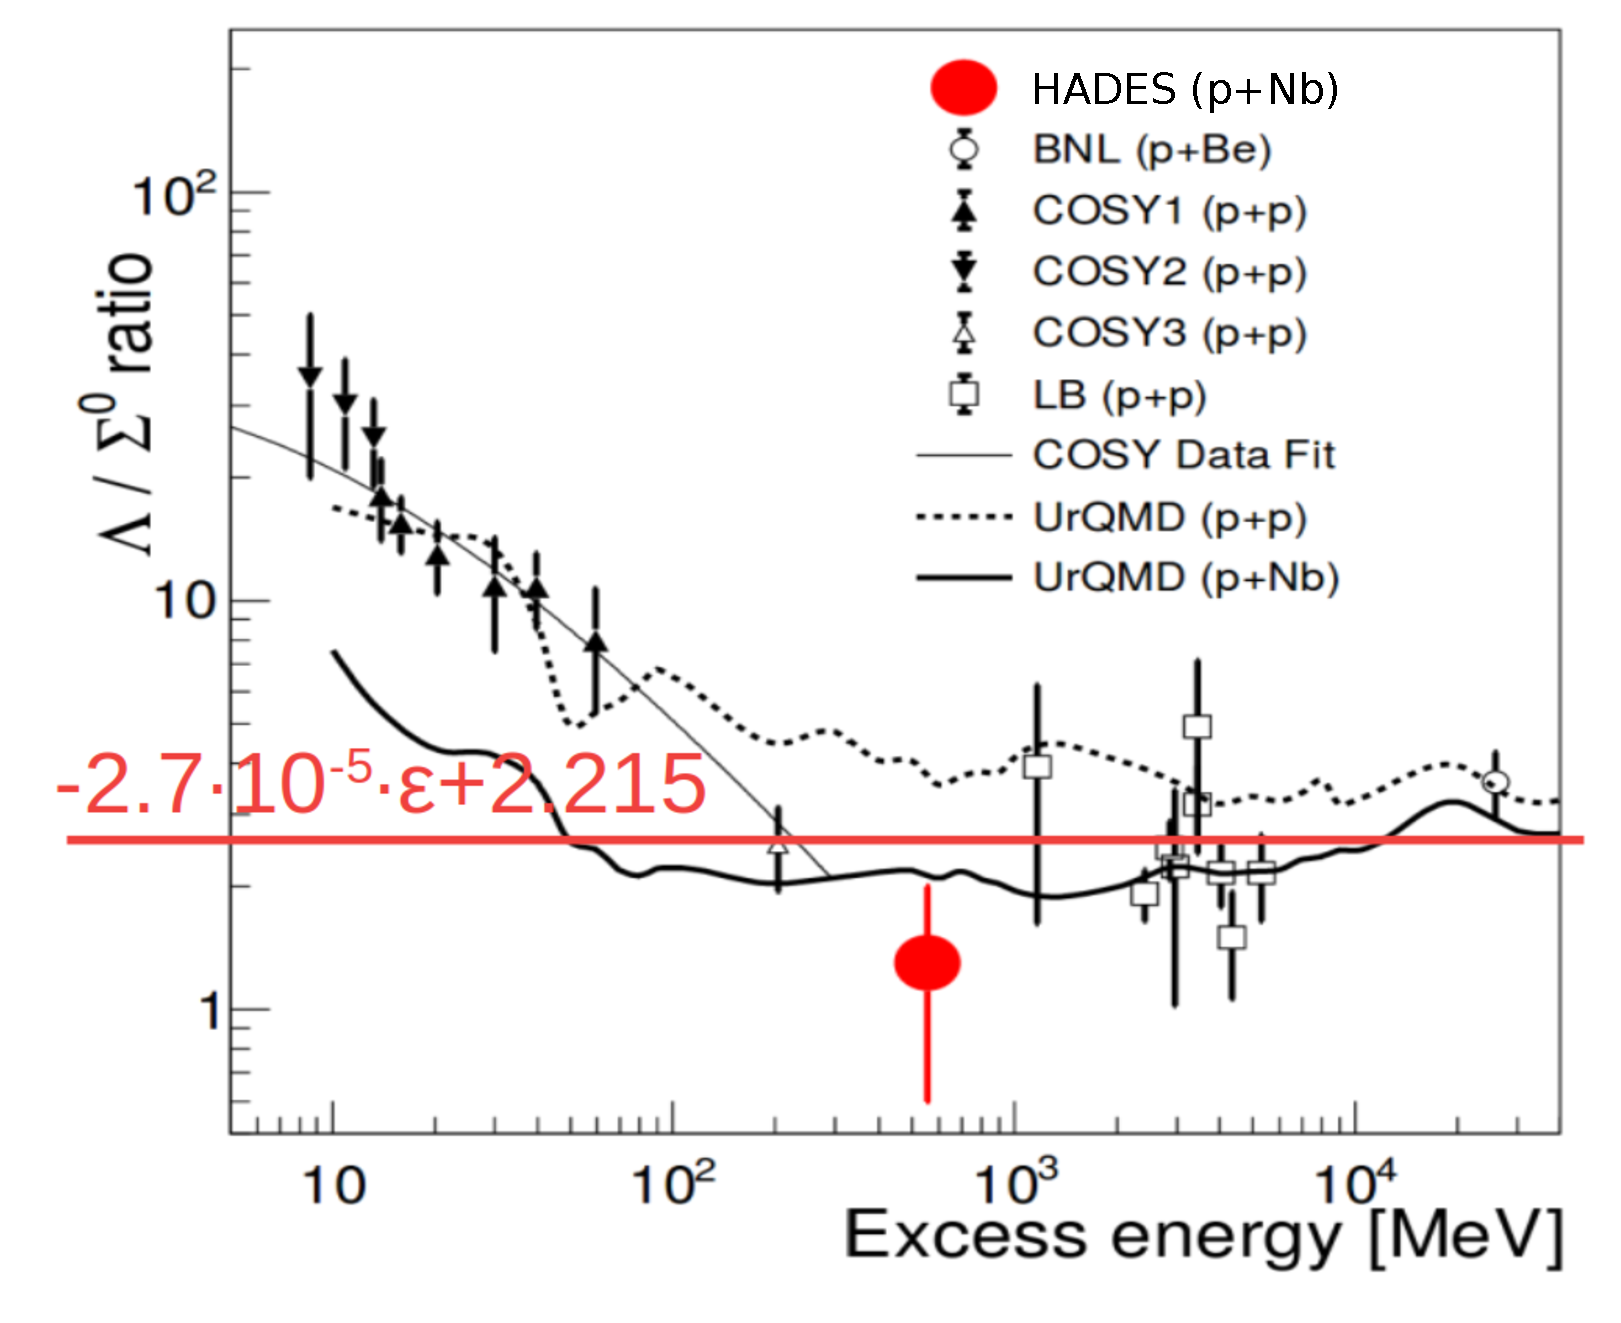
\includegraphics[width=0.6 \linewidth]{Chapter_simulation/LtoS.eps}
  \caption{A measeured ratio between $\Lz$ and $\Sz$ exclusive \cs. I low $\eps$ range the COSY-TOF parametrization was used, for $\eps > ???$ the data is described by liner function. The picture taken from \cite{hades_Sz_pNb}.}
  \label{fig:LtoS}
\end{figure}

A $\Sz/\Lz$ ratio was measured by COSY-TOF and others \cite{COSY-TOF_SigmaLambda}. Additionally the COSY-TOF collaboration proposed a parametrization of the ratio for access energy $\eps <200~\mathrm{MeV}$. Above this energy ($\eps >200~\mathrm{MeV}$) a linear parametrization 
\begin{equation}
  \frac{\Lz}{\Sz}(\eps)=2.215 - 2.7 \cdot 10^{-5} \eps
\end{equation}
describes data quite well ($\chi^2=0.89$). In fact for $\eps>200MeV$ the ratio is almost constant and does not depend on energy. For further calculations the COSY-TOF and the linear parametrizations were glued at ???.

Knowing the $\Lz/\Sz$ ration it is possible to disentangle a $\Lz$ and $\Sz$ production. Using determined ratio and the $\Lz$ production (let's call it~$P_1$) and  parametrization given by eq. \ref{eq:L1116param} (called~$P_2$), a following ste of equations is created 
\begin{equation}
  \label{eq:set_1}
  P_1(\eps)=\frac{L(\eps)}{\S(\eps)}=\frac{L(\Sqs - \Lz_{thr})}{\S(\Sqs - \Sz_{thr})}=P_1(\Sqs),
\end{equation}
\begin{equation}
  \label{eq:set_2}
  P_2(\Sqs)=\L(\Sqs)+\S(\Sqs),
\end{equation}
Where $\Sigma$ represents the inclusive $\Sz$ production \cs and  $\L$ the $\Lz$ \cs accordingly. Solving the first equation and shifting an argument by $\Sz_{thr}$ it is possible to obtain an equation,
\begin{equation}
  \label{eq:set_3}
  \S(\Sqs) \cdot P_1(\Sqs + \Sz_{thr})=\L(\Sqs - \Lz_{thr} +\Sz_{thr}).
\end{equation}
Now, using eq. \ref{eq:set_3} and \ref{eq:set_2} I got a recurrence relation
\begin{equation}
  \L(\Sqs - \Lz_{thr} +\Sz_{thr})=P_1(\Sqs +\Sz_{thr}) \left( P_2(\Sqs)-\L(\Sqs) \right).
\end{equation}
Assuming that $\L(\Lz_{thr})=0$ and $\S(\Sz_{thr})=0$, the above equation can be solved with any given precision. For the purpose of \css estimation a single step was set $\Delta M = \frac{\Sz_{thr}-\Lz_{thr}}{10}$, obtained decomposition is shown in \ref{fig:inclusive_cs} by dashed lines. A characteristic ``kick'' on the green line corresponds to energy when two parametrization of $\frac{\Lz}{\Sz}$ ratio are glued (see fig ??). 

\begin{figure}[hb]
  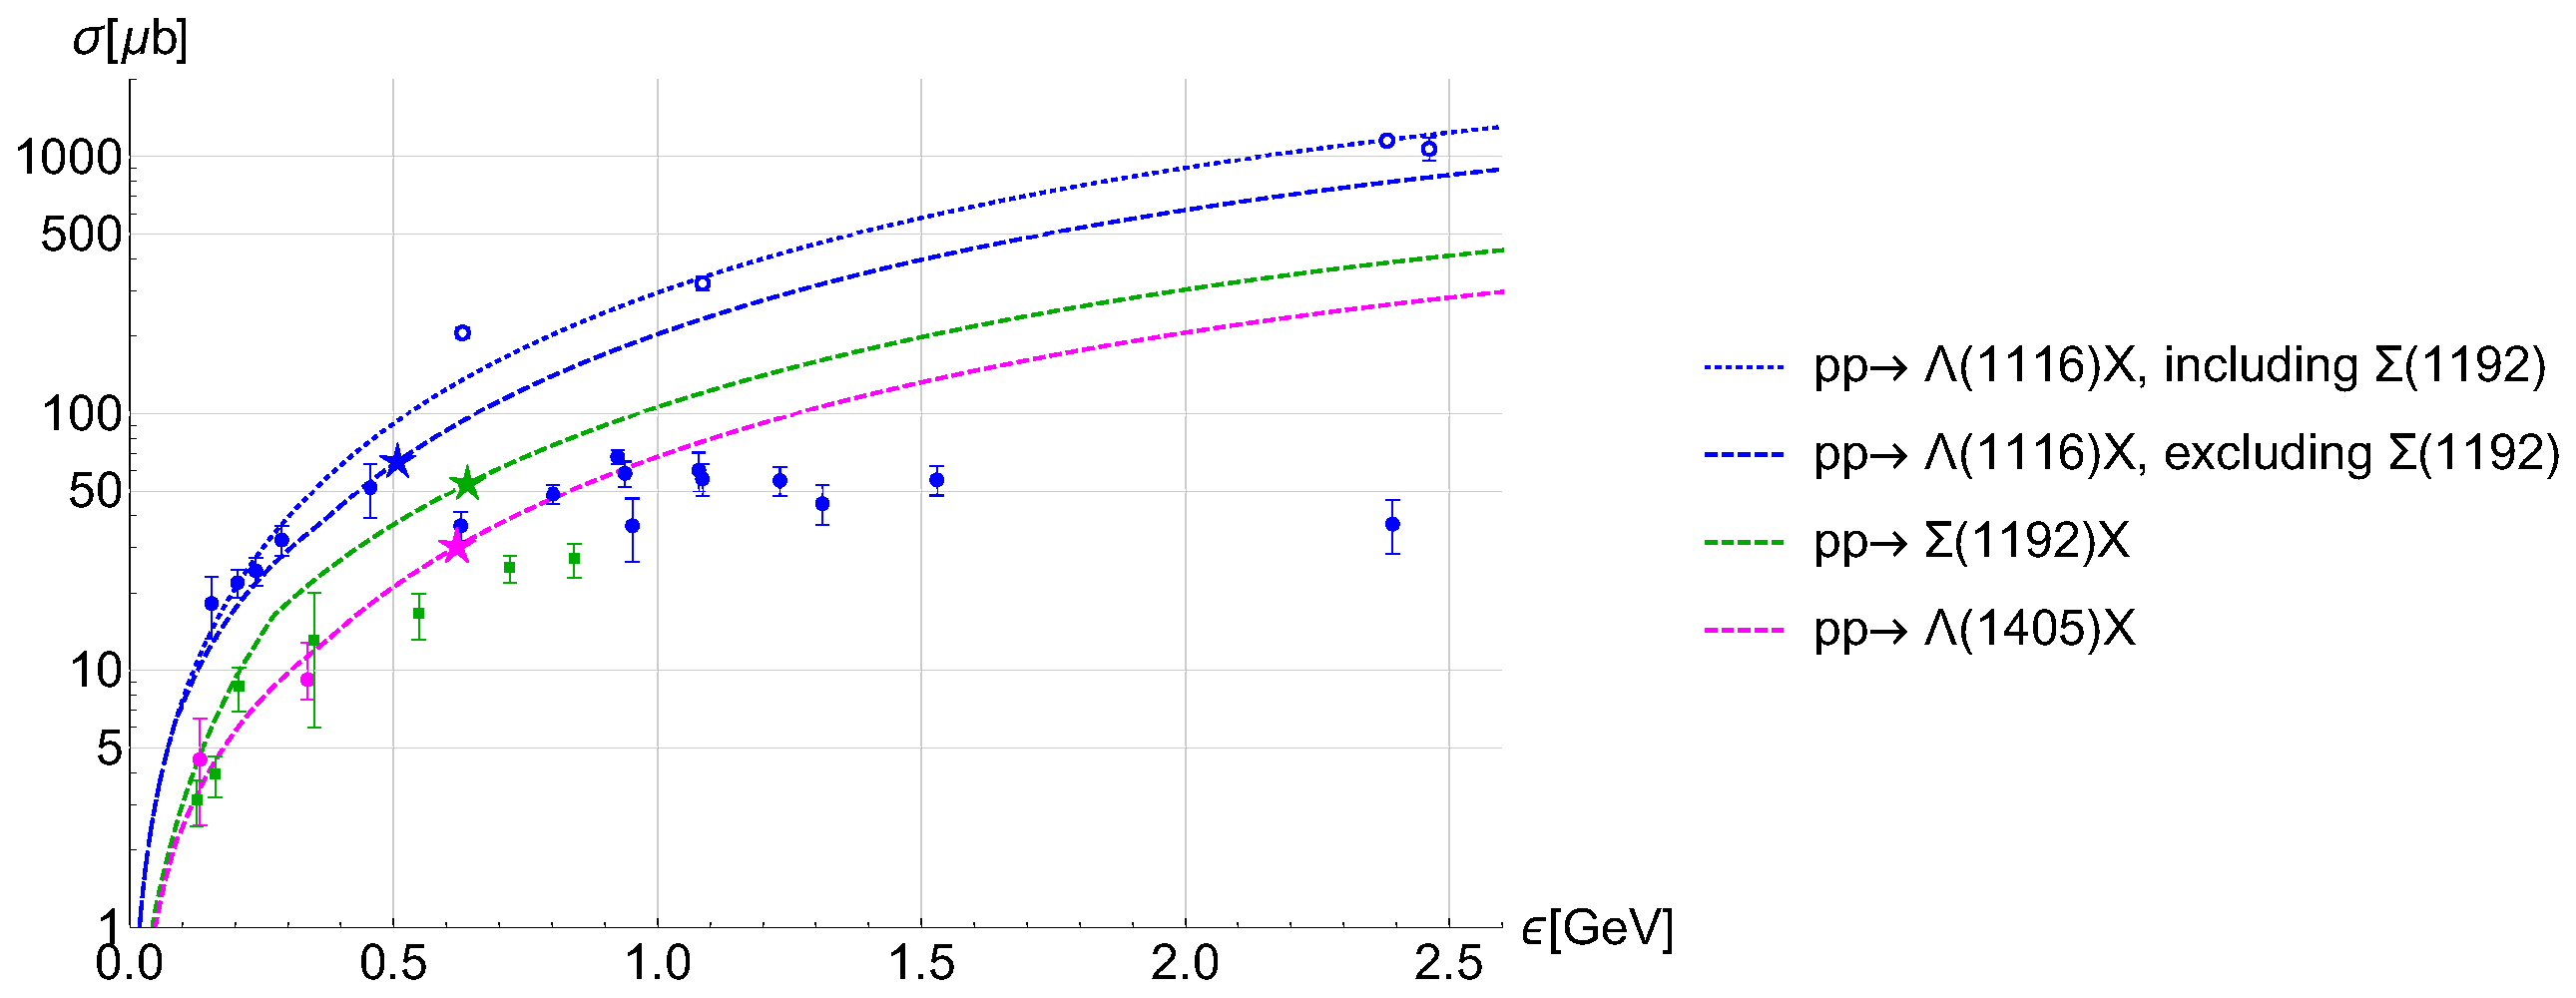
\includegraphics[width=0.9 \linewidth]{Chapter_simulation/all_CS}
  \caption{An estimated \css for Hyperons production. Blue dotted line shows an inclusive $\Lz$ production. It was decomposed into two components:i) $\Lz$ - blue dashed line and ii) $\Sz$ green dashed line. Magenta dashed line represents a parametrization of $\Lss$ \cs. All points refer to experimental data measured by different experiments \cite{L-B, COSY-TOF_L1405, COSY-TOF_SigmaLambda, hades_L1405, hades_inclL_35}. Color code is the same like for lines. Full points represent an exclusive \cs, empty points an inclusive one. }
  \label{fig:inclusive_cs}
\end{figure}

\subsection{$\Ls$, $\Lss$ and $\Ss$ production \css}
A knowledge about \css for $\L$ and $\S$ in function of $\Sqs$ or energy over the threshold $\e$ gives a possibility to estimate \cs for excited hyperon states. As a first approximation it was assumed that a production matrix element for ground and excited states is the same. It means that an only factor cases the difference in \cs is an avaliable energy over the treshold. It can be espressed by an equation
\begin{equation}
  \label{eq:cs_over_thr}
  \sigma_{\L^* X}(\L_{thr}^*+\eps)=\sigma_{\L X}(\L_{thr}+\eps),
\end{equation}
or in terms of $\Sqs$
\begin{equation}
  \sigma_{\L^* X}(\Sqs)=\sigma_{\L X}(\Sqs - \L^*_{thr}+\L_{thr}).
\end{equation}
Using the equation \ref{eq:cs_over_thr} I have calculated expected \css for the excided hyperons states $\Ls$ and $\Ss$. They are shown in \ref{fig:inclusive_cs} as blue and green star.  

A $\Lss$ exclusive \cs was mesured for two different energys by HADES \cite{hades_L1405} and COSY-tof \cite{COSY-TOF_L1405} experiment. In \cite{hades_L1405} outhors propozed a phenomentlogical parametrization of $\Lss$ exclusive \cs,
\begin{equation}
  \sigma^{excl}_{\Lss\p \Kp}(\eps)=\frac{1}{3}\sigma^{excl}_{\Lz \p \Kp}(\eps).
\end{equation}
I have followed the same relation for inclusive reactions multiplaying the inclusive $\Lz$ \cs by factor $1/3$. Result is shown in \ref{fig:inclusive_cs} by a magenta line. A magenta star shows point corresponding to $E_k=4.5 \mathrm{GeV}$ proton beam. Numerical values of the estimated \css are in tab. \ref{tab:sig_bg}.

\subsection{$\Xsi$}
Knowledge about a double-strange hyperon $\Xsi$ is extremly limited.
\section{Decay branching ratios}
Because Dalitz decays of hyperons were never measured a decay braching ratio have to be estimated considering avaliable data. A first approximation may be obtained using result for a non-strange sector. For a reaction $\Delta^+ \rightarrow \p \epem$ the HADES reported \cite{hades_Delta} $\mathrm{BR_{\Delta\rightarrow \p\epem}}=(4.19~\pm~0.62~\mathrm{~syst.}~\pm~0.34~\mathrm{~stat.})\times10^{-5}$. More precise estimation bases on, measured by CLAS collaboration \cite{Clas_Hyperons}, hyperons' radiative decays. A relation between radiative decays and Dalitz decays is given by the formula derived in F. Scozzi PhD thesis \cite{scozzi},
\begin{equation}
  \Gamma^{N^*\rightarrow~Ne^+e^-}=1.35 \cdot \alpha \Gamma^{N^*\rightarrow~N\gamma}.
\end{equation}
For $\Ls$ and $\Ss$ decay with for real photon decay are known. For $Lss$ the branchin ratio have to be astimted using other decay channels [ref]. Obtanied results (tab. \ref{tab:sig_bg}  are located in range of measured BR for $\Dp$ dalitz decay.


\section{Background channels selection}
To obtain a relaiablble simulation a coctail of background channels shoud be considered and tested. In case of hadronic physic, for low and medium enrgys, due to lack of approximation theorem, get a realistic background is a very challenging task. For a $\Sqs=$ 3.46 GeV a hadronic matter tends to form resonances. It means that almost all hadrons in final states originate from decays of high-mass resonances. Because knowledge about porperities of such a resonances is limited I made a simplified assumption that all pions are produced directly, without any intermediate state and with angular distribution defined jus by a reaction phase-space. List of all bacground channels considered during studies is presented in tab. \ref{tab:sig_bg}.

All channels considered as a $\Xsi$ background have to constist $\p \pim \pim$ in final state. A dominant one is a multi-pion production, however thanks to topological cuts (see chapter \ref{section:results}) this kind of the backgound is relatively easy to filter out. Second kind of the background considered in simulation is a $\Lz$ production associated with $\pim$. Reactions much more challenging because the $\Lz$ decay vertex is displaced from a target, the same like in signal reaction. \Css for channels numer 2-7 are taken from \cite{L-B}. When data in a proper energy range is missing, the value for the lowest avaliable enegry above $\Sqs=$ 3.46 GeV is taken. that conservative assumption gives me a save margin.

For all channels consisting of the hyperons' Dalitz decays a final state is the same: $\p \pim \epem$. That allows me to use the same background coctail for all three chanels. I divided possible bacground sources into three main grops. Firstly I considered a multi-pion production in a target area, channels: 14, 16 and 18. A di-lepton pair originates from a $\piz$ Dalitz decay and combination of $\p$ and $\pim$ creates false $\Lz$ signal. These channels differ from singal one mainly by a decay geometry. The $\Lz$ decays via week interaction with long lifetime $c\tau = 7.89$ cm \cite{PDG}, so its decay vertex is expected to be observed outside the target. A second group, channels 19, 21, 23, 24, 25, contains $\Lz$ production associated with a di-lepton source. In this case I have a real $\Lz$ and a $\epem$ pair coming from decay of different particles, mainly $\piz$. The \cs are taken from \cite{L-B}. The third source of background  are Dalitz decays of non-strange baryions associated with $\Lz$ production. The braching ratio was mesured only for $\Dp$ Dalitz \cite{hades_Delta}, for $\Dz$ Dalitz I have assumed the same value. A production \cs for the channels containing $\Delta$ has been calculated assumed that all pions comes from the reosnacnes decays. For example, channel 14 is the final state for reaction $\p\p \rightarrow p\Dp[\p\piz]\pip\pim$. Assuming that the $\Delta$ decay into pions conserv an izospin symmetry I used Clebsch-Gordan coefficients to calculate a ratio
\begin{equation}
  \frac{\Dp \rightarrow \p \piz}{\Dp \rightarrow \n\pip}=\frac{2}{1}.
\end{equation}
Hence, a total \cs for the reaction $\p\p \rightarrow p\Dp\pip\pim$ is $\frac{3}{2} \cdot \sigma_{pp \rightarrow \p\p \pip\pim\piz}$. The \css for other channels containing $\Delta$ dalitz decay were calculated in a similar way. Each $\Delta$ channel is listed below a reference multi-pion production channel. 

\begin{table}[!t]
  \centering
  \caption{List of signal (S) and background (B) channels for simulated reactions. Each channel containing $\Delta$ Dalitz decay is listed below reference channel, used for \cs estimation.}
  % \lineup
  \begin{tabular}{rlll}
    \hline
    no. &Channel & $\sigma$ [$\mu \barn$] & Type \\
    \hline
    \hline
    \multicolumn{4}{c}{$\Xsi$ production} \\
    \hline
    1&$\p\Kp\Kp\Xsi$                      & $\phantom{00}3.6/0.35$ & S \\
    \hline
    2&$\p\p\pip\pip \pim\pim$          & $\phantom{00}227$ & B  \\
    3&$\p\Lz\Kzs\pip$                  & $\phantom{00}30$ & B  \\
    4&$\p\Lz\Kp\pip\pim$               & $\phantom{00}21$ & B  \\
    5&$\neut\Lz\Kzs\pip\pip$           & $\phantom{00}10$ & B  \\
    6&$\p\Sz\Kzs\pip$                  & $\phantom{00}9$ & B  \\
    7&$\p\p\Kzs\Kzs$                   & $\phantom{00}1.6$ & B  \\

    %\multicolumn{4}{c}{$\dilambda$ production} \\
    %\hline
    %$\dilambda\Kp\Kp$                   & $\phantom{000}3.6/0.35$ & S \\
    %\hline
    %\multicolumn{4}{c}{background channels the same like for $\Xsi$ plus below} \\
    %$\p\p \Kp\Km$                    & $\phantom{00}20$ & B$^{\dagger}$ \\
    %\hline
    \hline
    \multicolumn{4}{c}{Dalitz decays of hyperons} \\
    \hline
    8&$\p\Kp\Ls[\Lz\epem]$          & $\phantom{0}69.6$, BR = \num{8.4e-5} & S \\
    9&$\p\Kp\Lss[\Lz\epem]$           & $\phantom{0}32.2$, BR = \num{5.3e-6} & S \\
    10&$\p\Kp\Ss[\Lz\epem]$           & $\phantom{0}56.24$, BR = \num{1.1e-4} & S \\
    \hline
    11&$\p\Kp\Ls[X]$                   & $\phantom{0}69.6$    & B  \\
    12&$\p\Kp\Lss[X]$                    & $\phantom{0}32.2$    & B  \\
    13&$\p\Kp\Ss[X]$                    & $\phantom{0}56.24$   & B  \\
    14&$\p\p \pip\pim\piz$              & $\phantom{0}1840$ & B \\
    15&$\p\pip\pim\Dp[\p\epem]$      & $\phantom{0}2760$, BR = \num{4.5e-5} & B  \\
    16&$\p\neut \pip\pip\pim\piz$          & $\phantom{0}300$      & B  \\
    17&$\p\pip\pip\pim\Dz[\neut \epem]$  & $\phantom{0}450$, BR = \num{4.5e-5} & B  \\
    18&$\p\p \pip\pim\piz\piz$          & $\phantom{0}300$      & B  \\
    19&$\p\Lz\Kp\piz$                   & $\phantom{0}43$      & B  \\
    20&$\Kp\Lz\Dp[\p\epem]$          & $\phantom{0}64$, BR = \num{4.5e-5} & B \\
    21&$\neut\Lz\Kp\pip\piz$               & $\phantom{0}20$      & B  \\
    22&$\pip\Kp\Lz\Dz[\neut\epem]$      & $\phantom{0}30$, BR = \num{4.5e-5} & B \\
    23&$\p\Lz\Kp\piz\piz$               & $\phantom{0}10$      & B  \\
    24&$\p\Sz\Kzs\pip$                  & $\phantom{0}9$      & B  \\
    25&$\p\Lz\Kp\piz\piz\piz$           & $\phantom{0}7$      & B  \\
    %\hline
    %\hline
    %\multicolumn{4}{c}{Real photon decays of hyperons} \\
    %\hline
    %$\p\Kp\Lss[\Lz\gamma]$        & $\phantom{00}69.6$, BR = \num{1.3e-2} & S \\
    %$\p\Kp\Ls[\Lz\gamma]$         & $\phantom{00}32.2$, BR = \num{5.0e-4} & S \\
    %$\p\Kp\Sstar[\Lz\gamma]$         & $\phantom{00}56.24$, BR = \num{1.1e-2} & S \\
    %\hline
    %$\p\p \pip\pim\piz$              & $\phantom{00}1840$    & B  \\
    %$\p\p \pip\pim\piz\piz$          & $\phantom{00}300$     & B  \\
    %$\p\Lz\Kp$                       & $\phantom{00}54.5$    & B$^{\ddagger}$ \\
    %$\p\Lz\Kp\piz$                   & $\phantom{00}43$      & B  \\
    %$\p\Lz\Kp\pip\pim$               & $\phantom{00}20$      & B  \\
    %$\p\Sz\Kp$                       & $\phantom{00}23.5$    & B$^{\ddagger}$ \\
    %$\p\Sz\Kp\piz$                   & $\phantom{00}20$      & B$^{\ddagger}$ \\
    %$\p\Sz\Kp\pip\pim$               & $\phantom{000}2$      & B$^{\ddagger}$ \\
    \hline
  \end{tabular}
  \label{tab:sig_bg}
\end{table}
\section{Simulations results}
The simulation has been performed usign folowing frameworks. The PLUTO event generator \cite{PLUTO1,PLUTO2} to simulate reactions in the target, the GEANT3 \cite{GEANT} software to simulate particles propagation through the detector and to simulate decay of unstable reaction's products like $\Lz$ or $\Kzs$. After all physics simulations, the detector answer and a full reconstruction chain was dane in the HYDRA framework. All together gives me a realistic simulation of an examineted physics, and the HADES behavour. The new HADES upgrades: new RICH, and the FwDet (see chapter \ref{chapter:HADES_upgrades}) were included.
\subsection{Particles identyfication}
\label{chapter:simulation_identyfication}
The particle identyfications algoritms used for simulation are, in principple, the same as for data collected during experiment. In first step all particle candidates are filtered to find events in wich track reconstracted in the MDC is fitted with the RICH rings. Additionally a Time-Of-Flight and Betha for leptonic track has to lay within a graphical cut. If both cryteria were fulfiled they are treated as lepton candidates. In next step for all non-leptnic candidates the mass is caltulated according to the formula
\begin{equation}
  m=\frac{pc}{\beta \gamma}.
\end{equation}
For protons and and pions the mass cuts are 650-1127 MeV and 40-240 MeV respectevly. 
\subsection{Hyperons Dalitz decays}

\subsection{Cascade decay}
\label{section:results}